% !TEX TS-program = pdflatex
% !TEX encoding = UTF-8 Unicode

% This is a simple template for a LaTeX document using the "article" class.
% See "book", "report", "letter" for other types of document.

\documentclass[11pt]{article} % use larger type; default would be 10pt

\usepackage[utf8]{inputenc} % set input encoding (not needed with XeLaTeX)

%%% Examples of Article customizations
% These packages are optional, depending whether you want the features they provide.
% See the LaTeX Companion or other references for full information.

%%% PAGE DIMENSIONS
\usepackage{geometry} % to change the page dimensions
\geometry{letterpaper} % or letterpaper (US) or a5paper or....
\geometry{margin=1in} % for example, change the margins to 2 inches all round
% \geometry{landscape} % set up the page for landscape
%   read geometry.pdf for detailed page layout information

\usepackage{graphicx} % support the \includegraphics command and options
\usepackage{hyperref}

\usepackage[parfill]{parskip} % Activate to begin paragraphs with an empty line rather than an indent

%%% PACKAGES
%\usepackage{booktabs} % for much better looking tables
\usepackage{array} % for better arrays (eg matrices) in maths
%\usepackage{paralist} % very flexible & customisable lists (eg. enumerate/itemize, etc.)
\usepackage{verbatim} % adds environment for commenting out blocks of text & for better verbatim
%\usepackage{subfig} % make it possible to include more than one captioned figure/table in a single float
% These packages are all incorporated in the memoir class to one degree or another...

%%% HEADERS & FOOTERS
\usepackage{fancyhdr} % This should be set AFTER setting up the page geometry
\pagestyle{fancy} % options: empty , plain , fancy
\renewcommand{\headrulewidth}{0pt} % customise the layout...
\lhead{}\chead{}\rhead{}
\lfoot{}\cfoot{\thepage}\rfoot{}

%%% END Article customizations

%%% The "real" document content comes below...

\title{Introduction to Arduino}
\author{ENGR 1624}
\date{} % Activate to display a given date or no date (if empty),
         % otherwise the current date is printed 

\begin{document}
\maketitle

%\begin{quote}
%Wise quote here.\\ \hbox{}\hfil -- {\em A Wise One}
%\end{quote}

\section*{Introduction}

Arduino is a common tool for introducing students to programming and prototyping with microcontrollers. With Arduino, the barriers to entry are very low, but the system can be made to do very powerful things. We don’t have time to cover much, but it will be useful for everyone on your team to be familiar with how to load and run code and the basics of programming.

In this exercise, you’ll build some circuits and learn some of the basic Arduino functions -- the building blocks, if you will -- of the Arduino environment. We’ll provide you with some skeleton code (i.e., code that is largely already written but still needs some meat on its bones) and ask you to change parameters and logical elements. For those that are interested in going further, sign up for the "Power to Control: Advanced Arduino" superpower.% For that, you’ll learn how to wire circuits and more advanced programming techniques.

\subsection*{Objectives}

Upon successful completion of this lab, a student will be able to:
\begin{itemize}
\item Build introductory circuits on a breadboard,
\item Edit and upload code to an Arduino,
\item Use basic Arduino routines to read sensors and control outputs,
\item Use the Serial Monitor to output data to a computer, and
\item Use an Arduino library, in this case the \verb|Servo| library.
\end{itemize}

\section*{Preparation}
\subsection*{Background materials}

Review the following materials:
\begin{itemize}
\item Read up on \href{https://learn.sparkfun.com/tutorials/what-is-a-circuit}{\underline{circuits basics}}. 
\item Read about \href{https://learn.sparkfun.com/tutorials/how-to-use-a-breadboard}{\underline{how to use a breadboard.}}
\item Download and unzip the sample codes needed for this lab as follows:
\begin{enumerate}
\item Download the \verb|arduino.basic| codes from github \href{https://github.com/gcl8a/arduino.basic}{\underline{here}}. Click on the "Clone or Download" button and download them as a .zip file.
\item If you haven't already, install the Arduino IDE. See instructions online.
\item Open the Arduino IDE find the "Preferences" under one of the menus. Find the location of your Sketchbook under Preferences and unzip the file you downloaded above into that location. Do not just move the .zip file there -- you may need to "extract" that file first if your operating system does not do that automatically (Windows typically does not).
\item Open the Arduino IDE and verify that the codes can be found under File $\rightarrow$ Sketchbook $\rightarrow$ arduino.basic.
\end{enumerate}
\textbf{You need to show up on Tuesday with the code ready to go!}
\end{itemize}

If you’re interested in learning more about some of the topics presented herein:
\begin{itemize}
    \item SparkFun has a \href{https://learn.sparkfun.com/tutorials/pulse-width-modulation}{\underline{decent tutorial about PWM}}.
    \item As well as a technical discussion of \href{https://learn.sparkfun.com/tutorials/analog-vs-digital}{\underline{analog vs. digital}}.
    \item \href{https://learn.sparkfun.com/tutorials/light-emitting-diodes-leds}{\underline{Way more than you'd ever want to know about LEDs}}.
\end{itemize}


\section*{I/O Fundamentals}

Physically, input and output with an Arduino happen through \emph{pins}, which aren’t actually pins but the sockets along the sides of the Arduino.\footnote{They’re called pins because the microcontroller chip -- the brains of the Arduino -- uses pins to communicate with the outside world.} Each of the pins is labelled (e.g., \verb|8| or \verb|A2| or \verb|GND|. Some of the pins have special functionality (you might have noticed a \verb|~| next to some of them), and we’ll explain some of that functionality in the tutorials (you must be on the edge of your seat...).

\subsection*{Digital output: Hello, World!}

As you saw in the background reading above, you can connect a pin on an Arduino to a circuit using a \emph{jumper wire}, a short piece of wire that has convenient, exposed ends that can be pushed into the Arduino or the breadboard. Here, you’ll first blink the built-in LED on the Arduino, and then you’ll build a circuit with a separate LED on your breadboard.

\subsubsection*{Procedure}

\begin{enumerate}
\item Connect the Arduino to your computer with a USB cable and open the Arduino IDE.
\item Navigate to Tools $\rightarrow$ Board and select ``Arduino/Genuino Uno" if it is not already selected.
\item Navigate to Tools $\rightarrow$ Port and select the port that corresponds to your device. On a Windows machine, it will likely show up as ``COM \#". On a Mac, it will likely have ``Arduino" or ``redboard" in the name. If it’s not obvious, just try one or call over an instructor. Better yet, unplug the Arduino, note which ports are in the list, plug the Arduino back in, and look for the new port.
\item Open the \verb|blink| example by selecting File $\rightarrow$ Sketchbook $\rightarrow$ arduino.basic $\rightarrow$ blink.
\item Upload the program by clicking the right facing arrow near the top-left of the IDE. The IDE will compile and upload the program, which starts running as soon as the upload is done. You should see the on-board LED on the Arduino blink on and off every second.
\end{enumerate}

Congratulations, you’ve now completed the “Hello, World!” equivalent of Arduino! Of course, blinking an on-board LED isn’t terribly useful, so let’s do something slightly less useless and build a circuit on a breadboard.

\subsubsection*{Procedure}

\begin{enumerate}
\item Disconnect the Arduino from your computer and build the circuit shown in Figure~\ref{fig:led}. 
\begin{itemize}
    \item It is always a good idea to disconnect the Arduino when building a new circuit to avoid any possibility of a short circuit.
    \item Note that the long leg of the LED should be connected to pin 13. This is the positive side of the LED. The negative side is marked not only by the shorter leg but also by the flat edge on the LED casing.
    \item For this circuit, you'll need the 330$\Omega$ resistor, which is marked with orange-orange-brown-gold stripes. For more on resistor sizing and markings (on your own time), \href{https://learn.sparkfun.com/tutorials/resistors/decoding-resistor-markings}{\underline{SparkFun has a good description}}.
\end{itemize}
\item Reconnect the Arduino. Since the code you loaded before lives in persistent memory, it will start running as soon as you connect the Arduino. You should see the on-board LED start to blink again, and if you did everything correctly, the LED on your breadboard will also blink.
\end{enumerate}

\begin{figure}[htbp]
\begin{center}
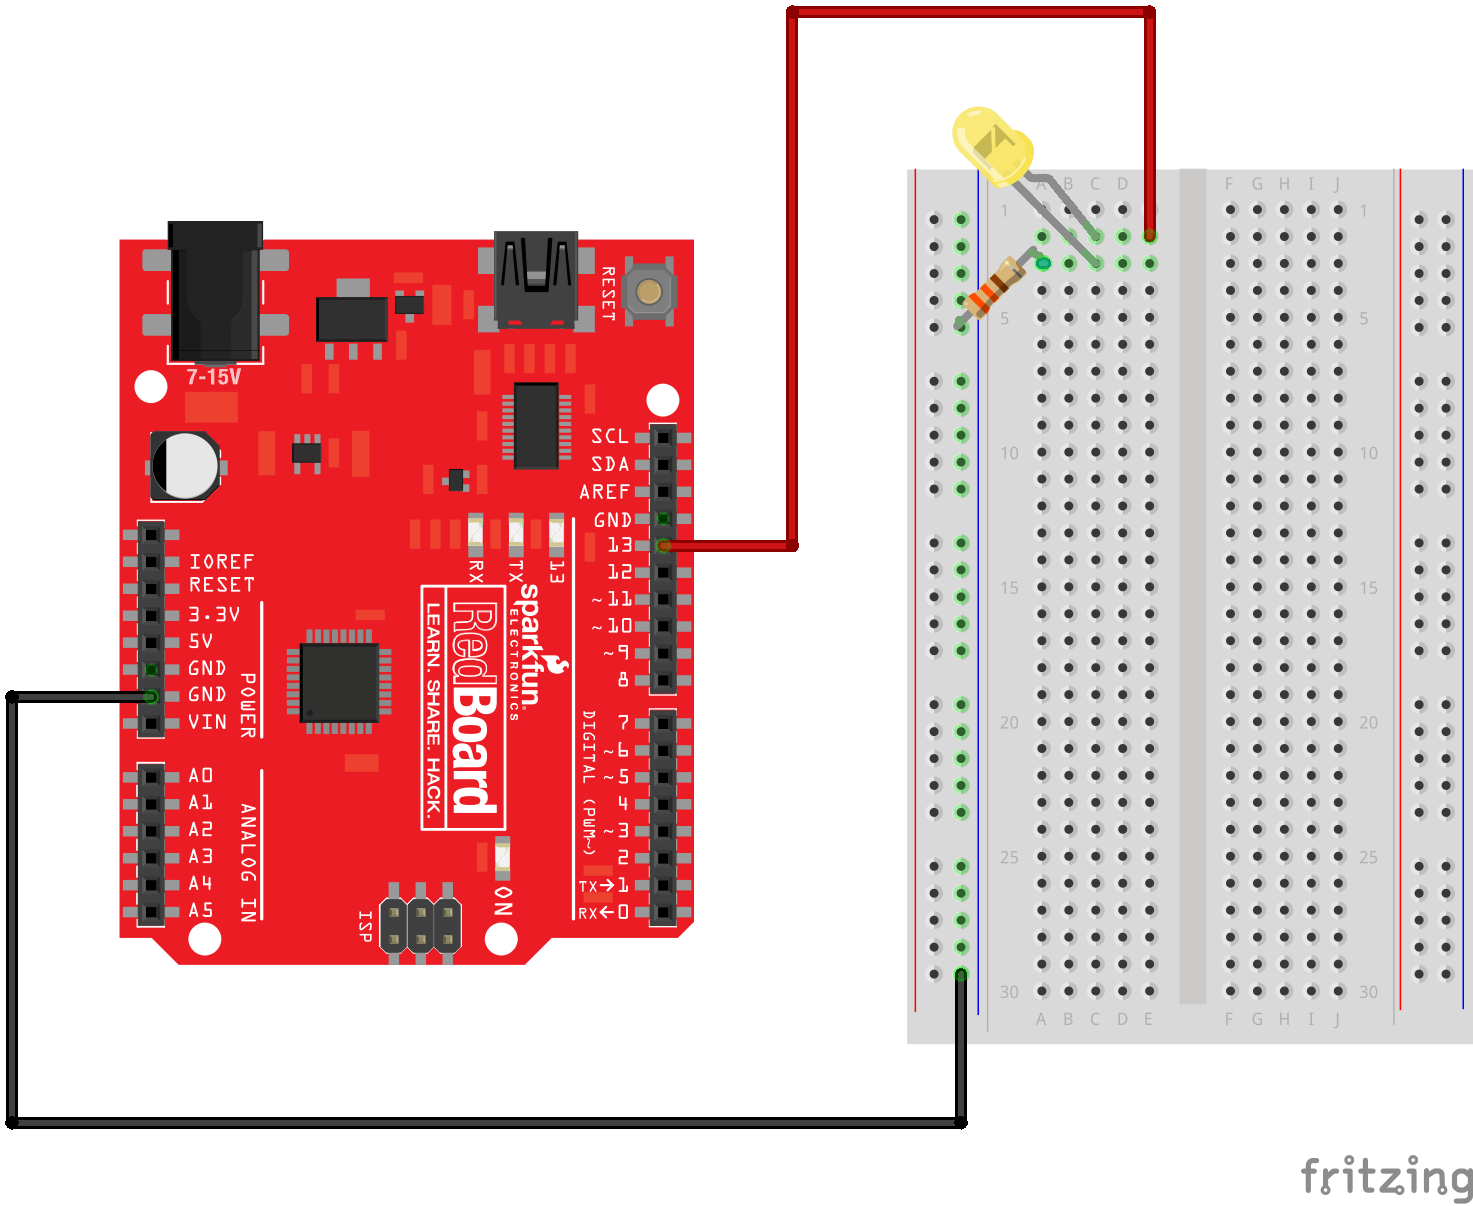
\includegraphics[width=4in]{figures/led_fritz.png}
\caption{Fritzing diagram for the LED breadboard circuit. }
\label{fig:led}
\end{center}
\end{figure}

%\clearpage

In a moment, you’ll make edits to the code, but first, let’s explain what the various lines of code are doing. Here is the complete program:

%\clearpage

\begin{verbatim}
const int ledPin = 13;

// the setup routine runs once at the start of the program:
void setup() 
{                
  pinMode(ledPin, OUTPUT);         // initialize the digital pin as an output.
}

// the loop routine runs over and over:
void loop() 
{
  digitalWrite(ledPin, HIGH);   // turn the LED on (HIGH is the voltage level)
  delay(1000);                  // wait for a second
  digitalWrite(ledPin, LOW);    // turn the LED off by making the voltage LOW
  delay(1000);                  // wait for a second
}
\end{verbatim}

The first line declares a variable, \verb|ledPin|, that will be used to tell the program which pin to use to control the LED. Capitalization matters, such that \verb|ledPin| is not the same as \verb|ledpin|.  To be able to control the pin, we must first set it to be an \verb|OUTPUT|, which typically happens in the \verb|setup()| routine. When you write a program using the Arduino IDE, everything in the \verb|setup()| routine will run \emph{once} when you first start the program. Everything in the \verb|loop()| routine will then run over and over, forever.

For example, in the \verb|loop()| routine above, the first line turns the LED on using the \verb|digitalWrite()| function. By writing \verb|HIGH| to \verb|ledPin|, the Arduino will make the pin output 5V and current will flow through the LED, turning it on. The code then waits 1000 \emph{milliseconds} using the \verb|delay()| command, after which it turns the LED off by setting the pin \verb|LOW|, followed by another \verb|delay()|. Because it’s in the \verb|loop()| routine, the code will be called over and over again. Lather, rinse, repeat. 

A few more syntax notes for those that are curious:
\begin{itemize}
\item The double forward-leaning slashes \verb|//| are used to denote comments. Anything after the double forward-leaning slahses are just comments that the computer does not read.
\item The semicolon after each line tells the computer that it is at the end of a statement.
\item The curly brackets before \verb|{| and after \verb|}| the \verb|setup()| routine and the \verb|loop()| routine tell the computer where the routines start and end.
\end{itemize}

Now you'll edit the code to change the length of time the LED is on and off.

\subsubsection*{Procedure}

\begin{enumerate}
\item Edit the code so that the LED will remain on for 2 seconds and turn off for half a second.
\item Upload the code and see if your code works as expected.
\end{enumerate}

{\bf Show your working system to an instructor.}

\subsection*{Digital input: Reading a button}

There are lots of things you can do with digital output: command motors to spin, make sounds, light LEDs, and a whole lot more. Of course, it’s also useful to \emph{input} signals into your microcontroller, for example, to read a button or (as you did in the sensor lab) a touch sensor. Here, you’ll declare a pin as an input and use it to detect the state of a button. When the button is down, the LED will light; when the button is up, it’ll turn off.

\textbf{Figure~\ref{fig:button} shows two buttons. You only need to build a circuit with one of those two buttons - your pick!!}

\subsubsection*{Procedure}

\begin{enumerate}
\item Disconnect the power to your Arduino and add one of the buttons as shown in the circuit shown in Figure~\ref{fig:button}.
\item Open the \verb|button| example code under Sketchbook $\rightarrow$ arduino.basic $\rightarrow$ button. Note the following:
\begin{itemize}
\item The button pin is declared as an \verb|INPUT|. This means it will respond to external signals that are applied to it.
\item When the button is not pressed, the  pins of the button are not connected electrically.  When it is pressed, the pins are connected electrically.
\item The button is connected to a 10$k\Omega$ resistor, which is marked with black-brown-orange-gold stripes. It is being uses as a \emph{pull-up resistor}, which guarantees that the button pin reads \verb|HIGH| when the button is \emph{not} pressed.
\item When pressed, the pin is connected electrically to ground so it will read \verb|LOW|. This is an example of \emph{inverted logic} because pressing the button makes the pin connected to the button \verb|LOW|. 

You could set this up with a \emph{pull-down resistor} if you put the resistor between ground and the button (instead of between 5V and the button), in which case an unpressed button would read \verb|LOW| and a pressed button would read \verb|HIGH|.  We'll only have you set it up as a \emph{pull-up resistor} during class today - but the concept is the same regardless.  If you are interested in learning more (outside of class), you can pull up or pull down \href{https://learn.sparkfun.com/tutorials/pull-up-resistors}{\underline{a great description here.}}
\item The pin is read using \verb|digitalRead(<pin>)|, which reads the state of the specified pin and returns a \verb|1| if the pin detects a \verb|HIGH| voltage and \verb|0| if it reads \verb|LOW|.
\item The result is then tested in an \verb|if..else| statement and the LED is set accordingly.
\end{itemize}
\item Make sure that \verb|buttonPin| corresponds to the physical pin on the Arduino that you connected to your button.
\item Upload the code and press the button to verify that the behavior is correct.
\item Edit the code so that the behavior is reversed: the light comes on when the button is up and goes off when pressed. Upload and test your code.
\item Now edit the code so that the program waits for 2 seconds after the button is pressed before turning that LED off. What function will you use? Upload and test your code.
\end{enumerate}

{\bf Show your working system to an instructor.}

\begin{figure}[htbp]
\begin{center}
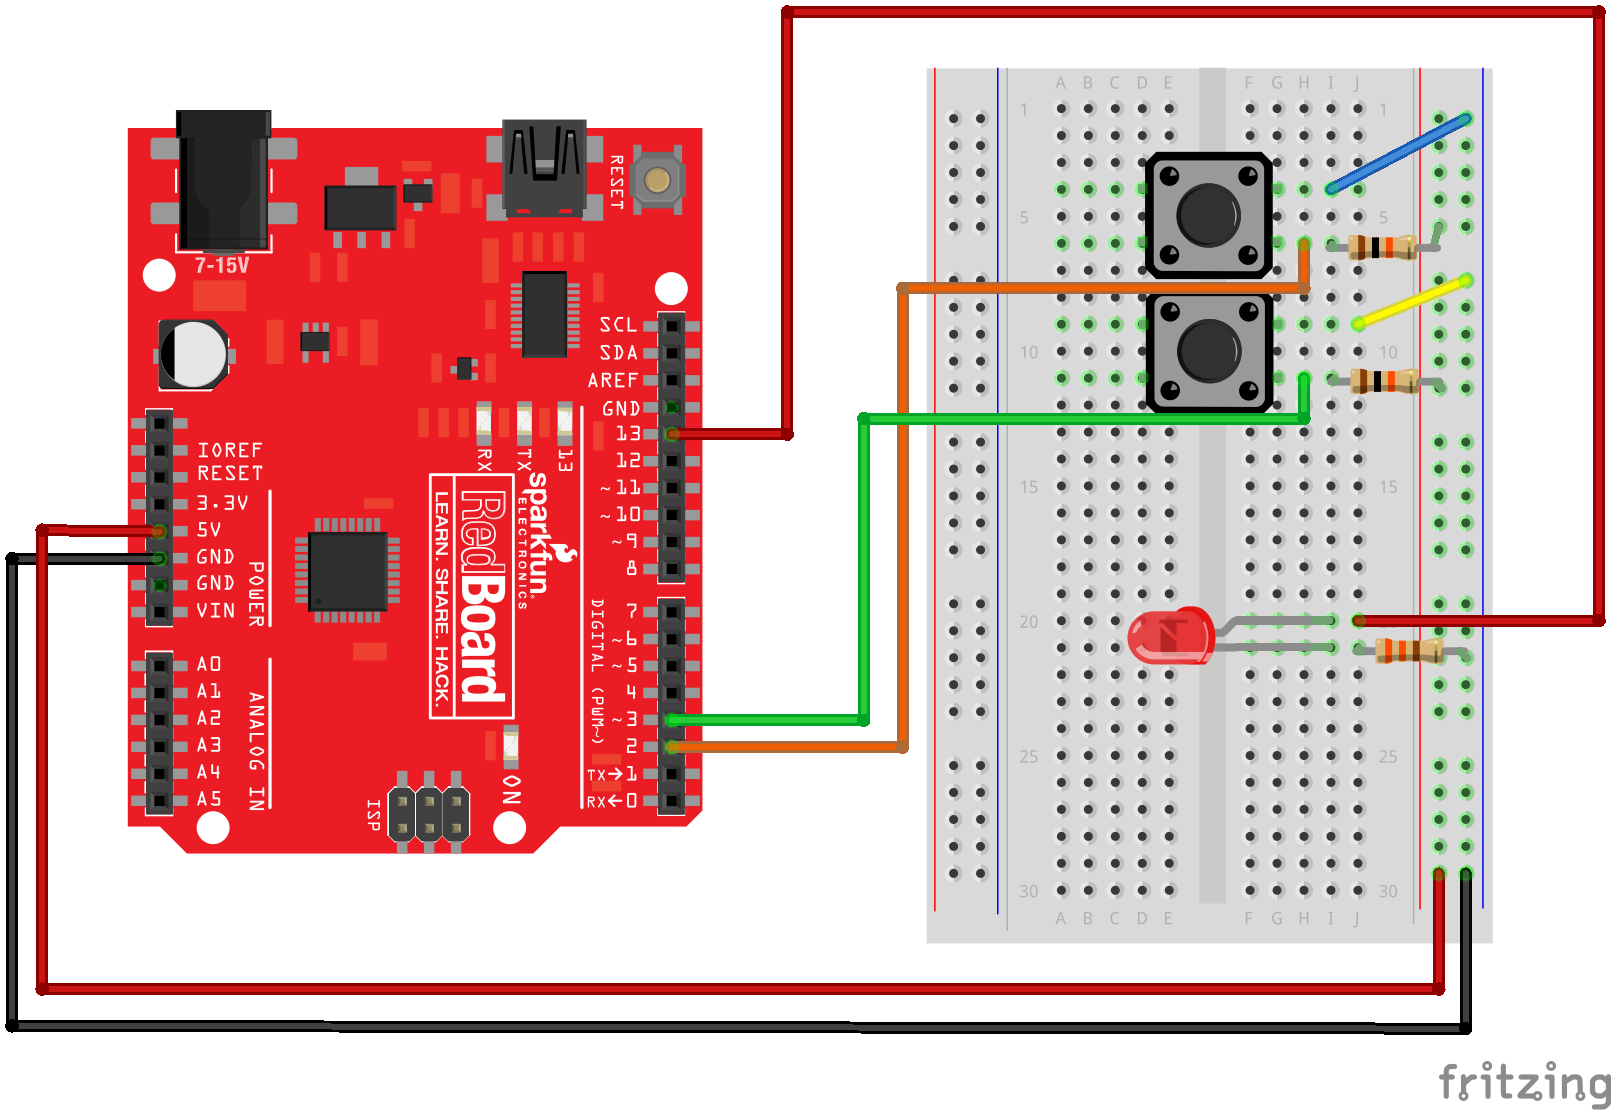
\includegraphics[width=4in]{figures/button_fritz.png}
\caption{Fritzing diagram for the button breadboard circuit. You only need to build the circuit for one of the buttons.}
\label{fig:button}
\end{center}
\end{figure}

\section*{Analog input and output}

Digital I/O, as demonstrated above, is extremely useful. However, there are times when you want to produce or read a signal that isn’t just \verb|HIGH| or \verb|LOW| -- some things are in between! For example, if you were controlling a motor, you might want to change the \emph{speed} of the motor, as opposed to just turning it on and off. Or perhaps you want to find the temperature, which is more than just “hot” or “cold”, but somewhere in between. For those functions, you need to use the \emph{analog} input and output functions.

\subsection*{Analog output: Dimming an LED}

Here, you will change the brightness of the LED using the \verb|analogWrite()| function. Just like \verb|digitalWrite()|, the function takes a \verb|pin| as an argument, but instead of \verb|HIGH| (5 V) or \verb|LOW| (0 V), you pass it a \verb|value| between 0 - 255, where 0 is off and 255 is fully on. Contrary to what the name suggests, however, the pin doesn’t actually vary the voltage of the pin directly. What it does is toggle the pin \emph{really fast} in a way that the \emph{average} voltage approximates an intermediate voltage. This apparent voltage is given by the formula:\footnote{If you're paying attention, you'll notice that this formula won't produce 0 V when you pass a 0 to analogWrite(). Arduino has special code to deal with this situation.}

\begin{equation}
apparent\ voltage = \frac{value+1}{256}\cdot 5 V
\end{equation}

%Figure~\ref{fig:pwm} shows a snapshot of the voltage on a pin at several different values for \verb|analogWrite()|. Notice how the width of the individual pulses grows as the value passed to \verb|analogWrite()| increases. 
Under the hood, the Arduino changes the \emph{duty cycle} -- the amount of time that the pin is on for each on-off cycle -- by varying the width of each 5 volt pulse. Figure~\ref{fig:pwm} shows an example of three different duty cycles. Because of this, the method of varying the apparent voltage is called \emph{pulse width modulation}, or just PWM. Note that the maximum value you can pass \verb|analogWrite()| is 255 -- values above that will have unexpected behavior.

\begin{figure}[htbp]
\begin{center}
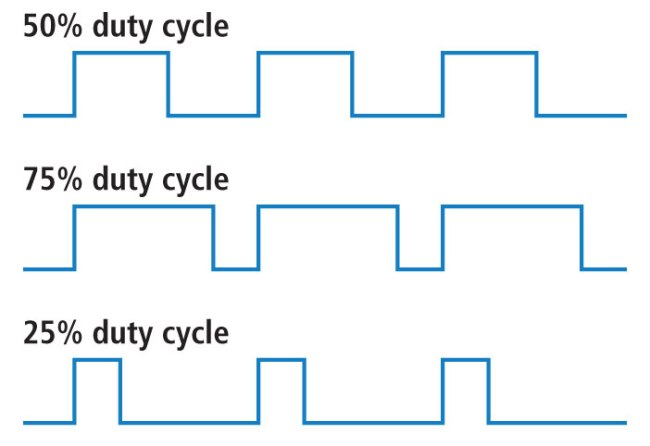
\includegraphics[width=4in]{figures/pwm.jpg}
\caption{Three different PWM duty cycles. Notice that the period of each cycle remains the same, but the width of the pulse is varied.}
\label{fig:pwm}
\end{center}
\end{figure}

\subsubsection*{Procedure}

\begin{enumerate}
\item Navigate to File $\rightarrow$ Save As... and save the current file (which should be \verb|button|) as \verb|dimmer|. While there are better ways to do code management, you don't want to clobber a working code that you're going to change, since you might need to go back to it to troubleshoot.
\item Move the wire that powers the LED from pin 13 to pin 11. Only the pins that have a \verb|~| next to them can perform PWM (the mystery of the \verb|~| is revealed!).
\item Change the line of code near the top to indicate that the led is on pin 11.
\item Upload the code to be sure that everything still works as before. \emph{It’s generally a good idea to change one thing at a time and test it, as opposed to changing a bunch of things all at once.}
\item Now change the \verb|digitalWrite()| statements to \verb|analogWrite()|. When the button is pressed, have the code pass a PWM value of 150 to \verb|analogWrite()|. Pass 75 when the button is up.
\item Upload the code. Press the button and notice what happens to the LED -- it should vary in brightness, but still be lit in both cases.
\end{enumerate}

{\bf Show your working system to an instructor.}

\subsection*{Analog input: Reading a potentiometer}

A potentiometer (which, in its rotary form as we use here, is a fancy name for a ``volume knob from a radio'') is a useful component when you want to have a variable control input. Unlike a button or a switch, which are either open or closed, the output of a potentiometer varies continuously. When connected as shown in Figure~\ref{fig:pot.sch}, the voltage produced on the middle pin, called the \emph{wiper}, will vary from 0 V to 5 V as the wiper moves back and forth along the resistive element.

\begin{figure}[htbp]
\begin{center}
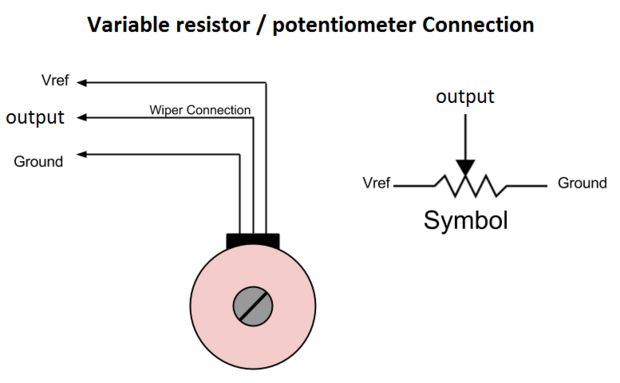
\includegraphics[width=4in]{figures/potentiometer.jpg}
%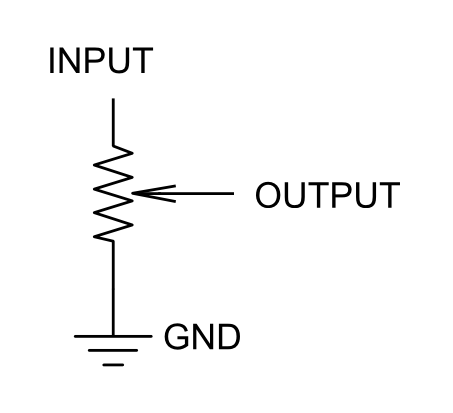
\includegraphics[width=2in]{arduino.basic/figures/divider-sym.png}
\caption{Physical representation and schematic symbol for a potentiometer. For an Arduino, $Vref$ is typically 5 V.}
\label{fig:pot.sch}
\end{center}
\end{figure}

To read this voltage, you’ll use something called an \emph{analog-to-digital converter}, or simply an \emph{ADC}, which converts a voltage into a value that can be used by the microprocessor. For an Arduino Uno, the ADC value is given by the formula:

\begin{equation}
ADC\ value = \frac{input\ voltage}{5\ V} \cdot 1024
\label{eq:adc}
\end{equation}

where the ADC value is rounded down to the nearest integer and constrained to be between 0 - 1023. For example, if the ADC were to sample 2 V, it would record a value of

\begin{equation}
ADC\ value = \frac{2\ V}{5\ V} \cdot 1024 = 409.6 \rightarrow 409
\end{equation}

%There is one caveat, however, which is that if you read 5 V with the ADC, it will output 1023 instead of 1024.

\subsubsection*{Procedure}
\begin{enumerate}
\item Unplug your Arduino and build the circuit shown in Figure~\ref{fig:pot}. The six analog pins, \verb|A0..A5| are used for reading analog voltages using the function \verb|analogRead(<pin>)|
\item Open the program \verb|potentiometer| from the same sketchbook location as before.
\item Upload and run the program. As you turn the potentiometer, the LED should grow brighter or dimmer, depending on which way you turn it.
\end{enumerate}

\begin{figure}[hbt]
\begin{center}
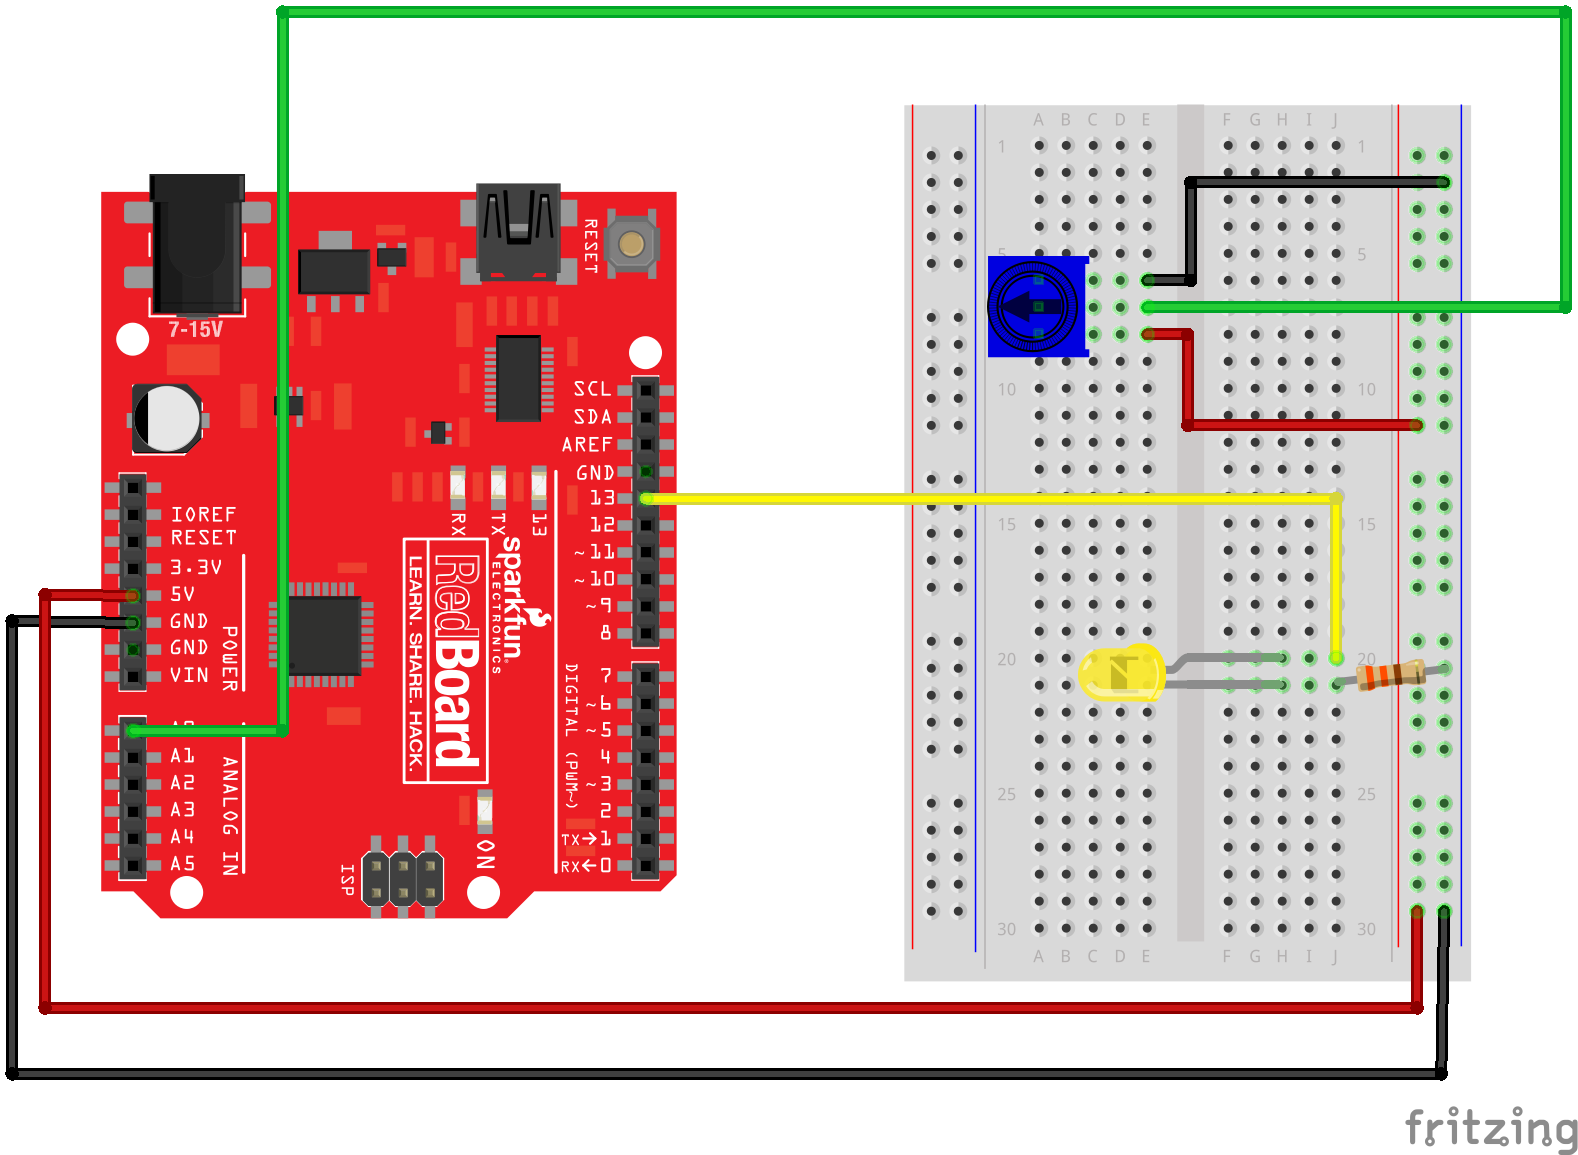
\includegraphics[width=4in]{figures/potentiometer_fritz.png}
\caption{Fritzing diagram for adding a potentiometer. Be sure to move the LED wire to pin 11.}
\label{fig:pot}
\end{center}
\end{figure}

Note that the result of \verb|analogRead()| is divided by 4 before the value is sent to the LED pin. While \verb|analogRead()| returns a value from 0 - 1023, as noted above, \verb|analogWrite()| only takes arguments from 0 - 255.

\subsection*{Analog input: Reading a temperature sensor}

Here you will determine the temperature in the room using a temperature sensor that outputs a voltage that varies depending on the temperature. Specifically, you will use the \verb|TMP36| temperature sensor, which outputs a voltage, $V$, according to the formula:

\begin{equation}
  V = 0.5 + 0.01 \cdot T
\end{equation}

where $T$ is the temperature in Celsius and $V$ is in volts.

In this program, you’ll make use of the Serial Monitor, which is a convenient way to send information from your Arduino to your computer. To use the Serial Monitor, you must call

\begin{verbatim}
  Serial.begin(<baud rate>);
\end{verbatim}

in your \verb|setup()| routine, where \verb|baud rate| is the speed that the Arduino will send data, in bits per second. Common choices are 9600 (the default) and 115200 (high speed). For these programs, it doesn’t matter which you use, \emph{just be sure to choose the same baud rate in the Serial Monitor when you open it}, otherwise you'll get gibberish. You write to the Serial Monitor using 

\begin{verbatim}
  Serial.print(<data>);
\end{verbatim}

and

\begin{verbatim}
  Serial.println(<data>);
\end{verbatim}

where the second version will send a newline character after it sends the data, causing the output to scroll. \verb|data| can be text or numbers, where the former must be enclosed in quotes, e.g.:

\begin{verbatim}
  float temperatureA = 22.5;
  float temperatureB = 30.1;

  Serial.print(”Temperature A = ”);
  Serial.println(temperatureA);
  Serial.print(”Temperature B = ”);
  Serial.println(temperatureB);
\end{verbatim}

would output:

\begin{verbatim}
  Temperature A = 22.5
  Temperature B = 30.1
\end{verbatim}

The \verb|float| denotes that a variable can have decimal places -- in computer-speak, it's referred to as a \emph{floating-point} number.

\subsubsection*{Procedure}

\begin{enumerate}
\item Unplug your Arduino and add the temperature sensor as shown in Figure~\ref{fig:tmp36}, \emph{except connect the middle leg of the sensor to pin} \verb|A1| (not pin \verb|A0| as shown in the figure). Leave the potentiometer in place for a later tutorial.
\textbf{NOTE}: The TMP 36 has a flat side and a rounded side on the black plastic housing. The flat side is facing to the right in Figure~\ref{fig:tmp36}.
\item Open the program \verb|tmp36|.
\item Upload and run the program. 
\item Start the Serial Monitor by clicking the magnifying glass in the upper-right of the IDE. The Serial Monitor will print out the value read by the ADC every second.
\item Using the formulas above, figure out the formulas to convert first from ADC value to voltage and then voltage to temperature.
\item Edit the lines of code that say \verb|float voltage = 0;| and \verb|float temperature = 0;| to compute the voltage and temperature using the formulas you just found. \textbf{Word of warning}: When coding the equations, use decimal points, e.g., \verb|adcValue / 1024.0|. This will tell the compiler to use floating-point math -- otherwise, the program will ``round" all the numbers and you'll end up with crazy results.
\item Add code to print the voltage and the temperature to the Serial Monitor, in addition to the raw ADC value that is already printed. Print each set of readings on one line, separated by a space. Add a delay of 500 ms after you print so that you don't overwhelm the Serial Monitor.
\item Upload the program and verify that your code works.
\end{enumerate}

{\bf Show your working system to an instructor.}

\begin{figure}[htbp]
\begin{center}
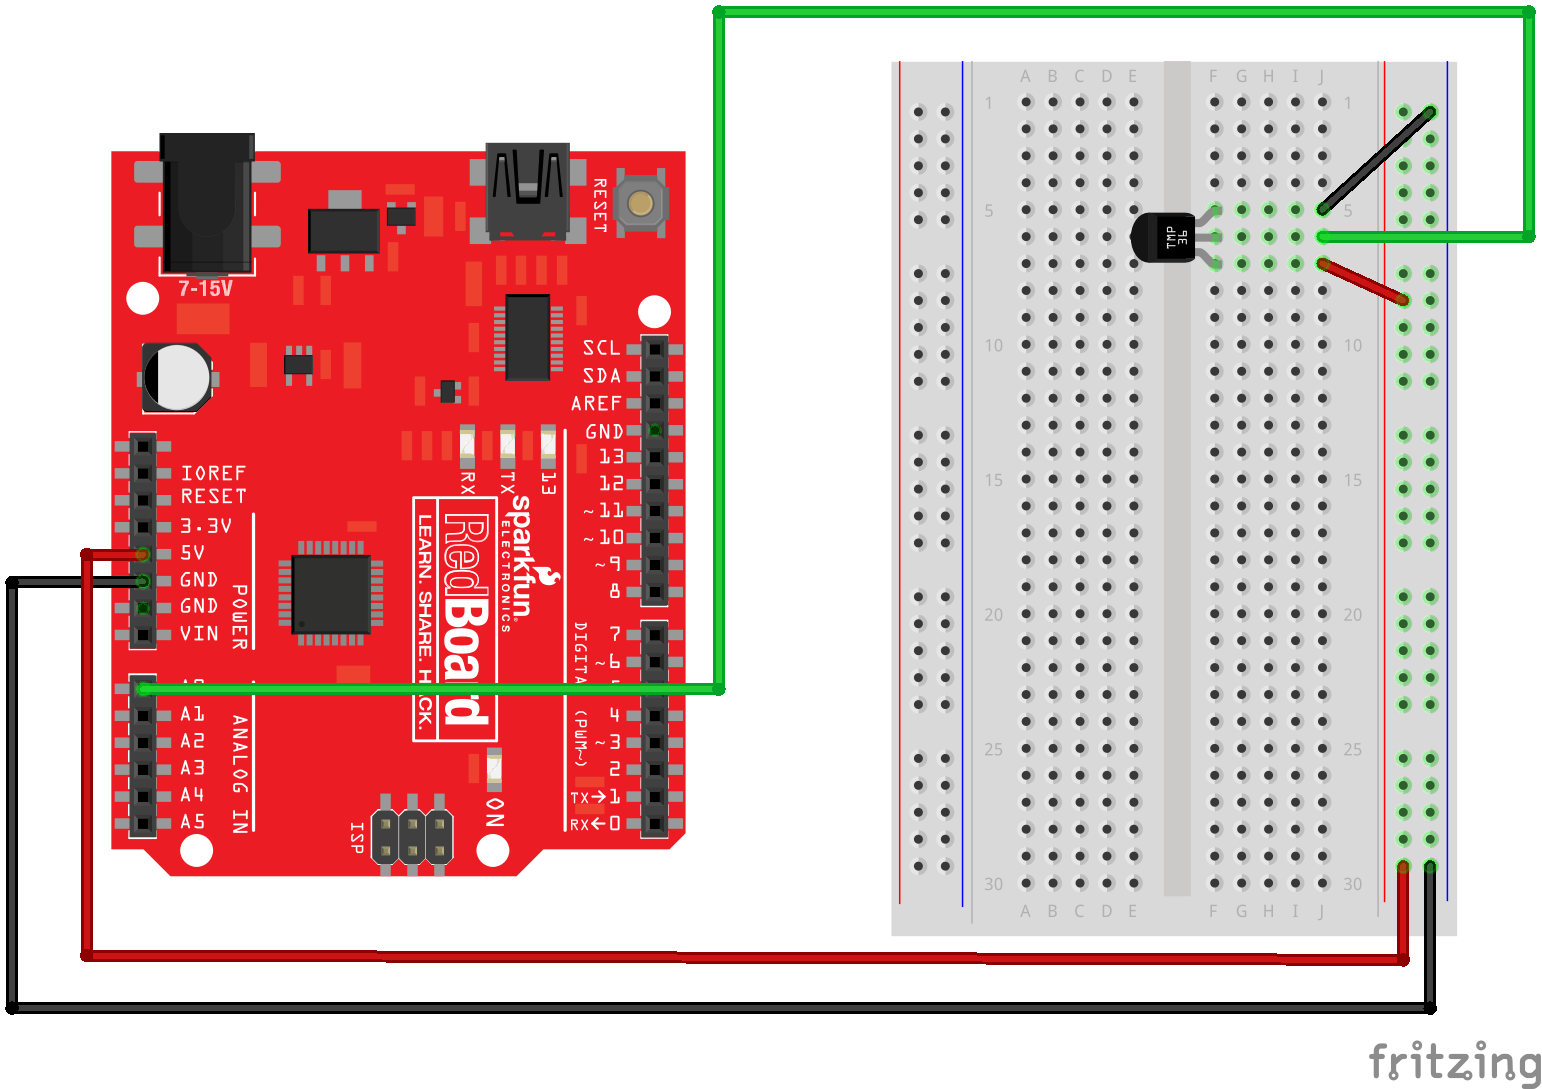
\includegraphics[width=4in]{figures/tmp36_fritz.png}
\caption{Fritzing diagram for adding the TMP36 tempearture sensor.  NOTE: the TMP 36 has a flat side and a rounded side on the black plastic housing.  The flat side is facing to the right in}
\label{fig:tmp36}
\end{center}
\end{figure}

\section*{Using libraries: Controlling an RC servo motor}

Kind people have written many libraries for Arduino to accomplish many common tasks: communicating with certain chips, connecting with WiFi or ethernet, running timers, and many, many more. The advantages of using existing libraries are obvious: no need to recreate code and flexibility topping the list. Be aware, however, that there are some disadvantages, as well; the most common one is that some libraries don’t “play nice” with others, which can lead to headaches. Here, we won’t concentrate on the pitfalls, but show how to implement and use a library, in this case the \verb|Servo| library. You’ll make a “dial thermometer” that shows the temperature by moving an RC servo motor.\footnote{It's referred to as an "RC servo" motor because this variety was made popular in remote control vehicle applications.}

\subsubsection*{Procedure}

\begin{enumerate}
\item Disconnect your Arduino from your computer and build the circuit in Figure~\ref{fig:servo}.
\item Open the example file \verb|knob|. This program reads the position of the potentiometer using the \verb|analogRead()| command and moves the servo in response to changes.
\item Near the bottom, there's a \verb|delay| statement. Depending on when you downloaded the code, this may be 15 ms or 200 ms. If your system doesn't work well at first, the first thing you should try is making the delay longer -- as much as 400 ms.
\item Connect the Arduino to your computer and upload the program. If all went well, you should be able to make the servo sweep back and forth in response to the turning of the potentiometer.
\end{enumerate}

\begin{figure}[htbp]
\begin{center}
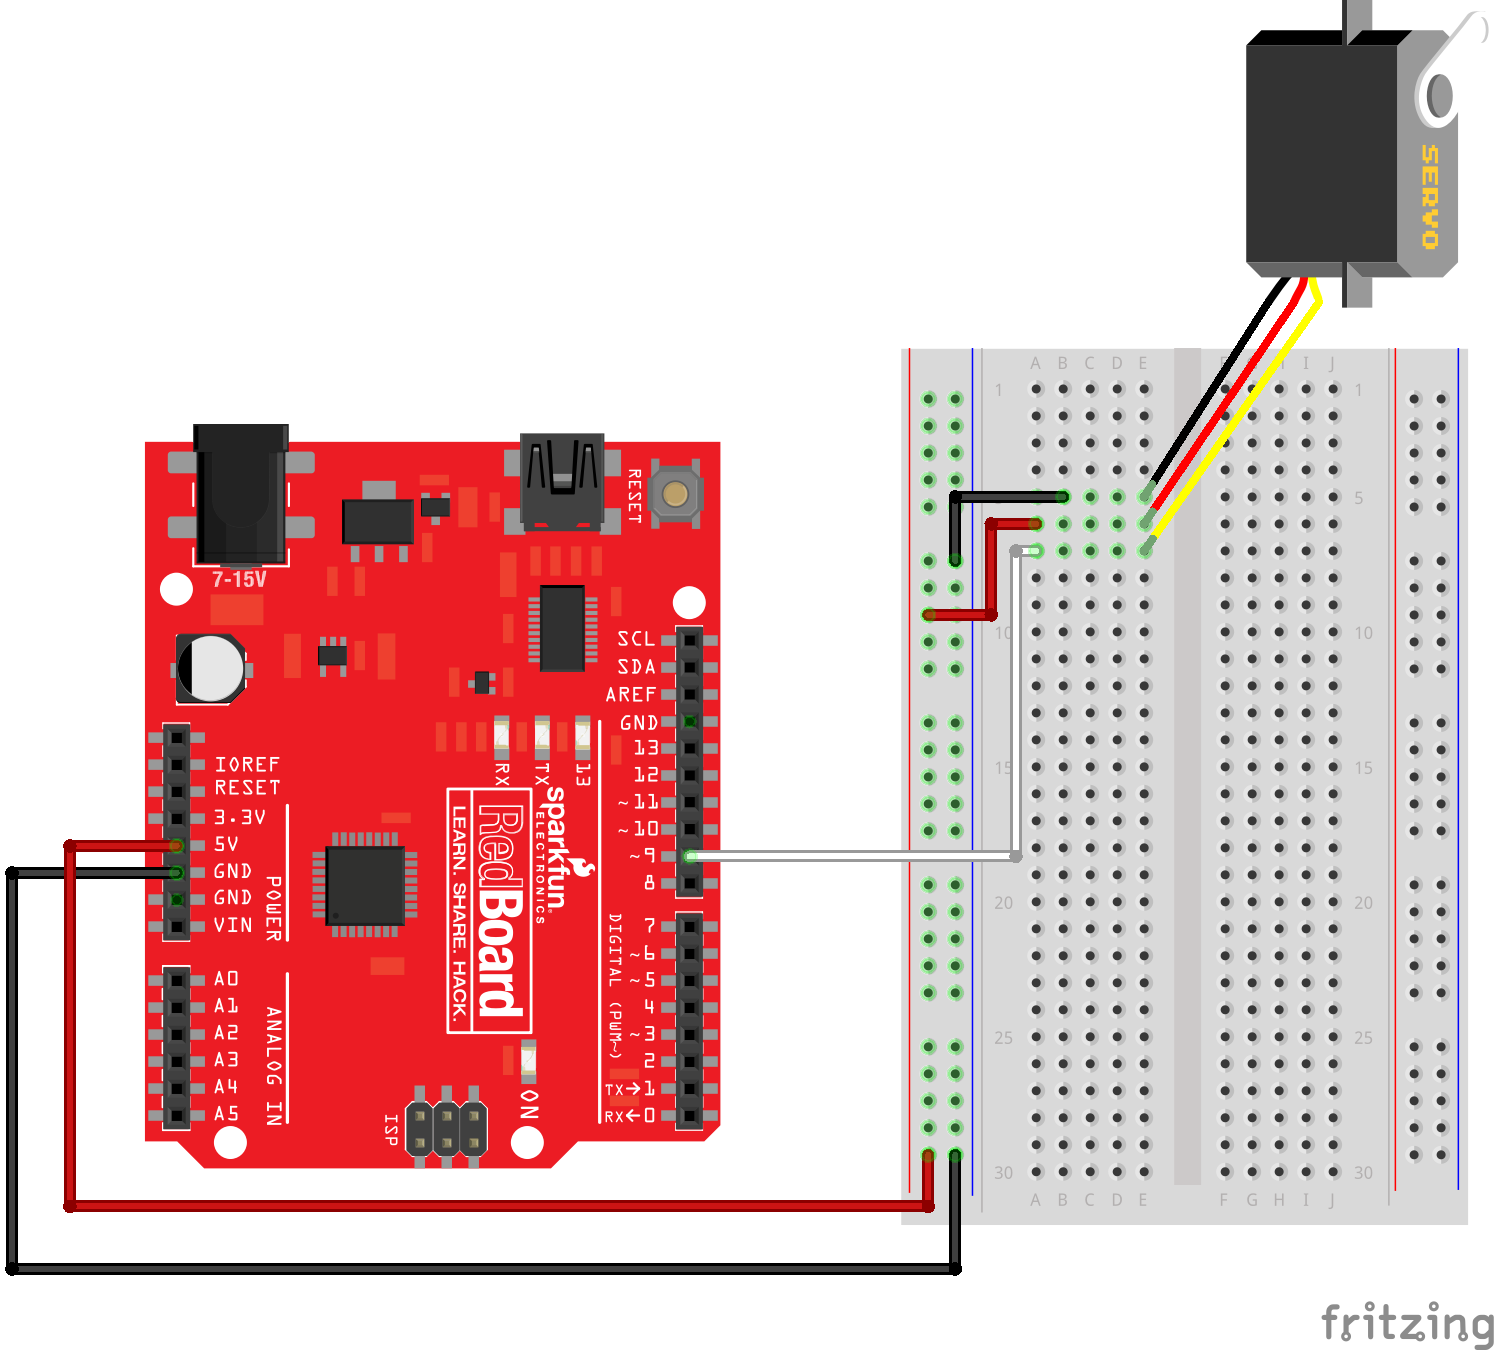
\includegraphics[width=4in]{figures/servo_fritz.png}
\caption{Fritzing diagram for adding the RC servo motor.  The potentiometer should already be there from earlier.}
\label{fig:servo}
\end{center}
\end{figure}

Before continuing, let’s explain what’s going on. There is some administrative work setting up the servo in \verb|setup()|. In the \verb|loop()|, the program reads the position of the potentiometer using \verb|analogRead()|. This value -- what is the range again? -- is scaled to a value of 0 - 180 using \verb|map()|, a convenient helper function, and the new value is used to command the servo using the \verb|Servo.write()| function, which takes an \emph{angle} (in degrees from 0 to 180) as an argument.

%\pagebreak

The Servo library has many useful functions. Let’s look at some details:

\begin{itemize}
\item Near the top of the code is a line that reads
\begin{verbatim}
#include <Servo.h>
\end{verbatim}
which tells the Arduino compiler to make use of the library. Other libraries are “\verb|#include|-d” similarly.
\item The command, \verb|Servo.attach(servoPin);| tells the Arduino which pin to use to talk to the servo motor (in this case, we set \verb|servoPin = 9| near the top of the program. A similar function, \verb|Servo.detach()| disconnects the servo.
\item One issue that is glossed over is the amount of power to drive the servo motor. Driving the servo from just the USB cable probably isn't going to give the servo enough power. If your servo jumps around a lot, you might want to use a separate power supply -- just ask and we'll find one for you. It helps to be a little cynical when it comes to Arduino tutorials -- easy is nice, but often there is more to the system than meets the eye. If you end up using a servo in your project, talk to us and we'll help you get set up with a separate power source for the servo.
\end{itemize}

Now, you’ll make your servo motor react to changes in temperature.
 
\subsubsection*{Procedure}

\begin{enumerate}
\item Start a new file under File $\rightarrow$ New. Call it \verb|thermometer|.
%\item Using your code from before, edit the code so that the servo position varies from 0 - 180 degrees over a temperature range of 20 - 35 C.
\item Add/edit code (you're welcome to cut-and-paste from the previous tutorials) so that your code has the following functionality:
\begin{itemize}
    \item It reads the temperature sensor and calculates the temperature in Celsius,
    \item It maps a temperature range of 20 - 35 C to an angle of 0 - 180,
    \item It commands the servo motor to move to that angle,
    \item It prints the raw ADC value, the temperature in C, and the position of the servo in degrees to the Serial Monitor. Print each record on one line, separated by spaces.
\end{itemize}
\item Upload and run your program. Place your fingers on the temperature sensor to show that warming the sensor will cause the servo to move in the expected way.
\end{enumerate}

{\bf Show your working system to an instructor.}
\end{document}

\clearpage
\section*{Lab worksheet}

To be handed in...

\begin{enumerate}
    \item Not sure if there is anything to turn in. Basically, if their systems work when shown to an instructor, they've done it.
\end{enumerate}

\end{document}
